\documentclass[11pt]{article}
\usepackage{fullpage}
\usepackage{graphicx}
\usepackage{subfigure}
\usepackage{comment}
\usepackage[utf8]{inputenc}
\usepackage{hyperref}
\usepackage{pdfpages}
\newcommand{\HRule}{\rule{\linewidth}{0.5mm}}

%numeroter les pages
\pagestyle{plain}

\renewcommand{\refname}{Références}
\renewcommand{\contentsname}{Table des matières}
\begin{document}

\begin{titlepage}

\begin{center}

% Upper part of the page

 


\includegraphics[width=0.8\textwidth]{./header}\\[1cm]
\textsc{\Large Stage Master Recherche}
\vspace{1cm}


\includegraphics[width=0.09\textwidth]{./logo_ENIB}

\includegraphics[width=0.1\textwidth]{./cerv}

\includegraphics[width=0.1\textwidth]{./CHRU-Brest}
%\includegraphics[width=0.1\textwidth]{./ens-Rennes}
%
\includegraphics[width=0.09\textwidth]{./esir}
%
\includegraphics[width=0.09\textwidth]{./enssat} 
%
\includegraphics[width=0.09\textwidth]{./insa-rennes}
%
\includegraphics[width=0.09\textwidth]{./rennes1}
%
\includegraphics[width=0.09\textwidth]{./supelec}
%
\includegraphics[width=0.09\textwidth]{./logoUbs}

\includegraphics[width=0.09\textwidth]{./UBO}

\includegraphics[width=0.09\textwidth]{./logo-labsticc}
%
\includegraphics[width=0.09\textwidth]{./tel-br}


  
\vspace{1cm} 
\textsc{\Large Rapport de stage }\\[0.5cm]


% The title of your report
\HRule \\[0.4cm]
{ \Large \bfseries Illusion de sortie de corps en réalité virtuelle pour \\l'anorexie mentale }\\[0.4cm]

\HRule \\[1.5cm]
% The domain of your research 
%\textbf{KEEP  WITHIN THIS LIST (see model.tex) ONE OR TWO DOMAIN(S) THAT CORRESPOND(S) TO YOUR INTERNSHIP - COMMENT OR REMOVE ALL THE OTHER ONES -}
\begin{flushleft}
\textbf{Domaine : Human-Computer Interaction - Emerging Technologies}
\end{flushleft}

\begin{comment}
Technology for Human Learning 
Artificial Intelligence 
Computer Arithmetic
Hardware Architecture
Automatic Control Engineering
Bioinformatics 
Biotechnology
Computational Complexity 
Computational Engineering, Finance, and Science
Computational Geometry 
Computation and Language 
Cryptography and Security 
Computer Vision and Pattern Recognition
Computers and Society 
Databases 
Distributed, Parallel, and Cluster Computing 
Digital Libraries
Discrete Mathematics 
Data Structures and Algorithms 
Embedded Systems 
Emerging Technologies 
Formal Languages and Automata Theory 
General Literature 
Graphics 
Computer Science and Game Theory 
Human-Computer Interaction 
Computer Aided Engineering 
Medical Imaging 
Information Retrieval 
Information Theory 
Ubiquitous Computing 
Machine Learning
Logic in Computer Science 
Multiagent Systems 
Mobile Computing
Multimedia
Modeling and Simulation 
Mathematical Software 
Numerical Analysis 
Neural and Evolutionary Computing 
Networking and Internet Architecture 
Operating Systems 
Performance 
Programming Languages 
Robotics 
Operations Research
Symbolic Computation 
Sound
Software Engineering 
Social and Information Networks 
Systems and Control 
Image Processing 
Signal and Image Processing 
Document and Text Processing
Web
\end{comment}
%
% Author and supervisor(s)
\begin{minipage}{0.4\textwidth}
\begin{flushleft} \large
\emph{Auteur:}\\
Guillaume  \textsc{Biannic}
\end{flushleft}
\end{minipage}
\begin{minipage}{0.5\textwidth}
\begin{flushright} \large
\emph{Superviseurs:} \\
%
% name(s) of your supervisor(s)
Cédric \textsc{Buche} \\ %of your first supervisor
Nathalie \textsc{Le Bigot} \\ %of your second supervisor  if any
% Name of your team
IHSEV - Lab-STICC
\end{flushright}
\end{minipage}

\vfill

\begin{comment}
% INCLUDE HERE THE LOGO OF YOUR INSTITUTION
\textbf{INSERT ``\%'' IN FRONT OF ALL THE LOGO YOU DO NOT NEED - A SINGLE ONE SHOULD REMAIN AT THE BOTTOM OF THIS PAGE}
\begin{flushleft}

\includegraphics[width=0.09\textwidth]{./supelec}\\
\end{flushleft}
\begin{flushleft}

\includegraphics[width=0.09\textwidth]{./logoUbs}
\end{flushleft}
\begin{flushleft}

\includegraphics[width=0.09\textwidth]{./UBO}
\end{flushleft}
\begin{flushleft}

\includegraphics[width=0.09\textwidth]{./tel-br}
\end{flushleft}
\begin{flushleft}

\includegraphics[width=0.09\textwidth]{./rennes1}
\end{flushleft}
\begin{flushleft}

\includegraphics[width=0.09\textwidth]{./insa-rennes}
\end{flushleft}
\begin{flushleft}

\includegraphics[width=0.09\textwidth]{./esir}
\end{flushleft}
\begin{flushleft}

\includegraphics[width=0.09\textwidth]{./enssat}
\end{flushleft}
\begin{flushleft}

\includegraphics[width=0.09\textwidth]{./ENS-Rennes}
\end{flushleft}
\end{comment}
\begin{flushleft}

\includegraphics[width=0.09\textwidth]{./logo_ENIB}
\end{flushleft}
\end{center}
\end{titlepage}



%************************************************************%

\thispagestyle{empty}
\section*{Abstract}
Les patients souffrant d'anorexie mentale ont une représentation faussée de leurs corps et surestiment leurs poids. Pour pouvoir soigner efficacement cette maladie, il faut aider le patient à prendre conscience de l'apparence de son corps. La réalité virtuelle a déjà permis d'aider les personnes atteintes de trouble du comportement alimentaire à améliorer l'image de leurs corps et pourrait donc aider efficacement ces patients. La sortie de corps est une illusion qui a déjà été réalisée en réalité virtuelle. Elle permet de faire croire à une personne que le corps virtuel qu'elle observe est son propre corps. Cette illusion peut être réalisée grâce à une corrélation visuotactile, lien entre ce qui est ressenti dans le réel et ce qui est vu dans le virtuel, et la corrélation visuomotrice, lien entre les mouvements réalisés dans le réel et ce qui est vu dans le virtuel. Le but de ce projet est de mettre au point une méthode et une application utilisable par les psychiatres pour aider au soin des personnes atteintes d'anorexie mentale. Nous nous sommes appuyés sur les travaux traitants de la sortie de corps et de la modification de la perception du corps, pour proposer une application basée sur l'illusion de sortie de corps et la modification de modèles d'humain virtuel pour répondre à notre problématique tout en respectant les contraintes liées à notre contexte applicatif. Nous avons également défini une méthode pour évaluer le travail réalisé.


%Cette illusion peut être réalisée à partir de stimulation tactile mais elle pourrait peut-être également être créée si le corps virtuel reproduit les mouvements de l'utilisateur. Le but de ce projet est de produire la sensation de sortir de corps puis de modifier la silhouette du corps virtuel : initialement le corps virtuel est telle que le patient se perçoit et se transforme jusqu'à sa silhouette réelle. Pour cela il faut donc pouvoir modifier l'apparence du corps virtuel avec une technique comme la \emph{shape interpolation}. Il faut également être en mesure de capturer les mouvements réalisés par le patient pendant la sortie de corps pour bouger le corps virtuel avec le minimum de délai afin de ne pas briser l'illusion.
%\end{abstract}


% compile twice to get the table of contents
\tableofcontents
\thispagestyle{empty}
\setcounter{page}{0} 
\newpage


%*****************************************************************%
\section{Introduction}

Ce rapport va vous décrire le stage de master recherche informatique que j'ai réalisé au CERV (Centre Européen de Réalité Virtuelle) au sein de l'équipe IHSEV. Ce projet est réalisé en collaboration avec le département de psychologie de l'UBO et le CHU de Brest. Le but est de mettre au point une méthode et une application qui pourront, à terme, être utilisées par les psychiatres pour aider au soin des personnes atteintes d'anorexie mentale.\\

L'anorexie mentale est une maladie grave qui touche principalement les femmes à l'adolescence. Les personnes atteintes de cette maladie se voient plus grosses qu’elles ne le sont même si elles ont atteints un faible poids corporel ce qui interfère avec le traitement des patients. Pour pouvoir soigner cette pathologie, il faut corriger cette erreur de perception. Certaines solutions ont été mise en place comme des sessions d'exposition face à un miroir lors de thérapie. Mais cela prend du temps car même face à un miroir, l'erreur de perception persiste et il faut donc recommencer cela régulièrement. L'utilisation de massage peut également aider ces personnes, mais il se peut que cette méthode les rende mal à l'aise dû à la nature de leur maladie.\\

Il a déjà était montré que la réalité virtuelle peut aider à soigner les troubles du comportements alimentaire et les problèmes d'images du corps \cite{ri11}\cite{ri13}. \`{A} présent, les environnements virtuels peuvent provoquer des réponses émotionnelles et comportementales similaires à celles qui peuvent être provoquées par le monde réel. Cela permet également de fournir un environnement sûr où la personne peut avoir moins de réticence à interagir et également plus flexible permettant de créer des mises en situation plus facilement que dans la réalité.\\

Avec la réalité virtuelle, on peut créer le sentiment qu'un corps virtuel est notre vrai corps, qu'il nous appartient, grâce à un phénomène connu sous le nom de sortie de corps en réalité virtuelle. Cette technique peut également permettre de changer la perception qu'une personne a de son corps grâce à l'apparence du corps virtuel.\\

En utilisant la sortie de corps, on pourrait alors donner aux patients la sensation que le corps virtuel est leur vrai corps puis modifier en temps réel la silhouette de ce corps. Le patient choisira le corps virtuel (parmi plusieurs) dont l'apparence est la plus proche de ce qu'il perçoit comme son apparence puis, en même temps que le phénomène de sortie de corps est créé, on modifiera progressivement la silhouette du corps virtuel jusqu'à ce qu'elle soit proche de la véritable silhouette du patient.\\

Pour pouvoir réaliser cela, il faudra d'abord être capable de pouvoir modifier l'apparence d'un modèle 3D de corps humain en temps réel. Il faudra également capturer les mouvements de l'utilisateur pour animer en temps réel le corps virtuel afin de ne pas "briser" l'effet de sortie de corps, voire même s'en servir pour créer cette effet.\\

Dans une première partie, nous étudierons des travaux déjà réalisés sur l'anorexie mentale, la sortie de corps, la modification de modèle 3D et la capture de mouvement. Ensuite nous verrons en détails ce que nous proposons pour répondre à la problématique et comment nous l'avons réalisée. Puis nous verrons l'expérience mise en place pour tester notre travail. Pour finir, nous verrons les modifications qui pourraient être apportées.


\section{\'{E}tat de l'art}

\subsection{Contexte}

Dans cette partie, nous allons voir ce qu'est l'anorexie mentale et ce qui a été réalisé dans le domaine de la sortie de corps en réalité virtuelle. Pour finir, nous verrons les contraintes à respecter pour créer une illusion en sortie de corps en réalité virtuelle pour aider les personne atteintes d'anorexie mentale.
\subsubsection{Anorexie mentale}

L'anorexie mentale est une maladie faisant partie des troubles du comportement alimentaire. Il s'agit une maladie psychiatrique grave qui touche principalement les femmes au moment de l'adolescence suite à une perte de poids et se présente essentiellement sous la forme de trois symptômes :
\begin{itemize}
\item Une restriction alimentaire entraînant une réduction drastique des apports énergétiques malgré les besoins physiologiques.
\item Une peur importante de reprendre du poids.
\item Une mauvaise représentation de son corps.
\end{itemize}

Les personnes touchées par cette maladie surestiment leur poids et leur silhouette, ce qui stoppe ou ralentit le processus de renutrition. Pour déterminer la source de cette mauvaise représentation du corps, Guardia et al. \cite{gu10} ont mis en place une expérience dans laquelle une personne est face à un mur sur lequel est projeté une porte dont la largeur varie. La personne doit alors dire si elle peut passer la porte sans tourner les épaules. Cette expérience a été faite sur des personnes en bonne santé et des personnes atteintes d'anorexie mentale. Ils ont pu observer que les personnes souffrant d'anorexie mentale se tournaient bien avant les autres personnes. Ces résultats tendent à indiquer que le schéma corporel, qui est une représentation sensorimotrice du corps sollicité pour gérer la posture et les actions du corps, serait faussé chez les patients.\\

 Comme le schéma corporel est supposé être basé sur une intégration multisensorielle, l'illusion de la main en caoutchouc ("\emph{Rubber Hand Illusion}") \cite{Bo98} (Voir Figure \ref{fig1}), qui se base sur la création de conflit dans le processus d'intégration multisensorielle, a été réalisée sur des patients souffrants d'anorexie mentale. L'illusion a pour but de faire croire à la personne que la main en caoutchouc fait partie de son corps. Pour cela, une des mains de la personne est cachée et une main en caoutchouc est placée devant elle. Ensuite, la main cachée et la main en caoutchouc sont touchées, par un bâton ou un pinceau par exemple, simultanément ce qui provoque un conflit entre ce qui est vu, la main en caoutchouc touchée par un pinceau, et ce qui est ressenti, la sensation de toucher créée par le pinceau sur la main cachée. Une fois l'illusion créée, on peut ne caresser que la main en caoutchouc. Cette illusion s'est avérée très forte chez les personnes atteintes d'anorexie mentale.\\

Pour aider les patients souffrants d'anorexie mentale, il faut d'abord les aider à corriger la mauvaise représentation qu'ils ont de leurs corps. Pour cela il faut pouvoir modifier la perception qu'ils ont de leur corps. L'illusion de la main en caoutchouc permet de le faire uniquement sur une partie du corps mais elle est très efficace sur eux. Donc la sortie de corps qui repose sur le même principe que cette illusion mais en l'étendant à tout le corps devrait également être efficace sur les personnes atteintes d'anorexie mentale.
\begin{figure}[h]
   	\centerline{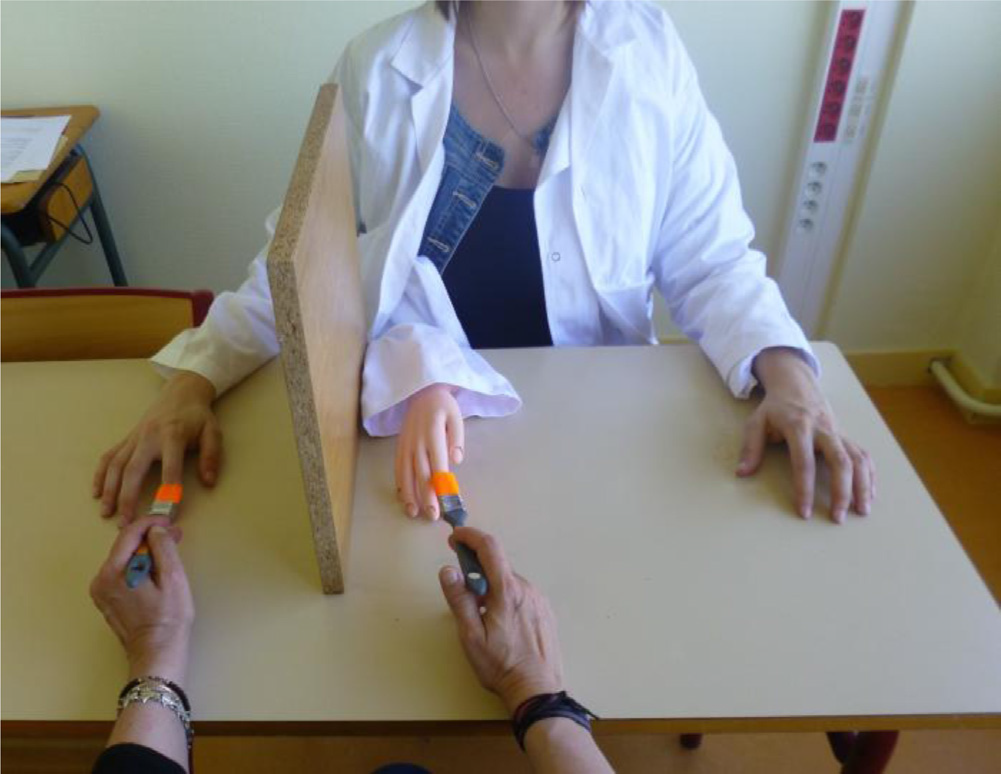
\includegraphics[scale=0.4]{images/biblio/rubberhand}}
   	\caption{\label{fig1} Illusion de la main en caoutchouc \cite{lu14}}
\end{figure}


\subsubsection{Sortie de corps}

La sortie de corps est un phénomène dans lequel une personne a l'impression d'apercevoir le monde d'une position surélevée et de voir son corps à l'extérieur de ses limites physiques, d'avoir la sensation d'être désincarnée \cite{bl10}. Dans cette partie nous allons voir différents travaux réalisés pour reproduire ce phénomène en réalité virtuelle. En réalité virtuelle, l'illusion de sortie de corps cherche à créer une sensation d'appartenance d'un corps ou une partie de corps virtuel contrairement à la vrai sortie de corps qui se définit par une désincarnation.

\paragraph{Sortie de corps en réalité virtuelle}

Olaf Blanke et al. \cite{le07}, se sont appuyés sur l'illusion de la main en caoutchouc pour mettre au point leur expérience (voir Figure \ref{fig2}). Dans cette expérience, le sujet porte un casque de réalité virtuelle et est filmé de dos. Le film est envoyé en temps réel au casque porté par la personne ce qui fait qu'elle voit donc une image de son corps projeté devant elle. Le sujet est alors touché à répétition dans le dos par un bâton. Il voit alors une image virtuelle dans laquelle le dos de son corps est touché par un bâton et en même temps ressent une sensation de toucher dans le dos. L'expérience est réalisée dans deux conditions, une où l'image est synchronisée avec la stimulation tactile et une autre où un délai est ajouté pour créer un décalage entre le moment où la personne est touchée par le bâton et le moment où elle se voit touchée par le bâton dans son casque de réalité virtuelle. Avec la synchronisation, les sujets avaient l'impression que la sensation de toucher venait du fait que le corps virtuel qu’ils percevaient via le casque était touché par un bâton. \'{E}galement, en demandant aux sujets, après qu'ils se soient déplacés, de se remettre à la position où ils étaient, ils avaient tendance à se placer plus près de là où leur corps virtuel était projeté qu'il ne l'était en vrai. Ceci tend à montrer qu'ils se sont identifiés au corps virtuel. Par contre, dans le cas où il n'y avait pas de synchronisation, ces erreurs d'assimilation étaient plus rares.\\

Simuler une attaque sur le faux corps, avec un couteau ou un marteau, peut même augmenter la conductance de la peau ce qui montre une réponse émotionnelle lorsque le corps virtuel est menacé \cite{eh07}. Le même résultat a pu être obtenu en filmant un mannequin de dos touché par un bâton au lieu de filmer directement la personne de dos, même si dans ce cas-là il faut aussi que le sujet soit également touché dans le dos de manière synchronisée par rapport au mannequin \cite{le07}.\\

\begin{figure}[h]
   	\centerline{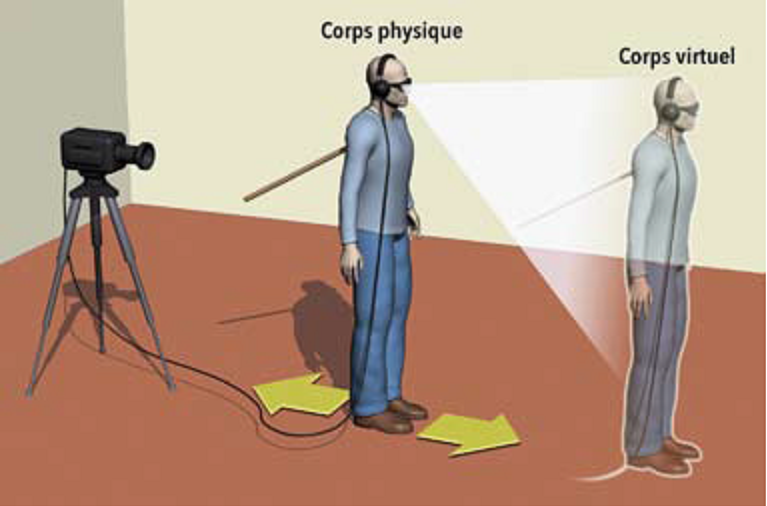
\includegraphics[scale=0.6]{images/biblio/oobRV}}
   	\caption{\label{fig2} Exemple de sortie de corps en Réalité Virtuelle \cite{bl10}}
\end{figure}

L'illusion de la main en caoutchouc a également était réalisée en réalité virtuelle \cite{sl09}, et elle a été réalisée sans utiliser de stimulation tactile mais en bougeant la main virtuelle pour qu'elle reproduise les mouvements de la main de la personne \cite{sl08}(Voir Figure \ref{fig3}). En utilisant un gant de données pour reproduire les mouvements de la main et des doigts de la personne, ils ont pu constater une tendance à identifier la main virtuelle comme étant une partie du corps. La synchronisation entre les mouvements réalisés par le sujet et ceux fait par la main virtuelle est importante pour créer ce sentiment d'appartenance. Cela permet de penser qu'une sortie de corps pourrait être réalisée en reproduisant le mouvement de la personne sur un avatar virtuel.


\begin{figure}[!h]
   	\centerline{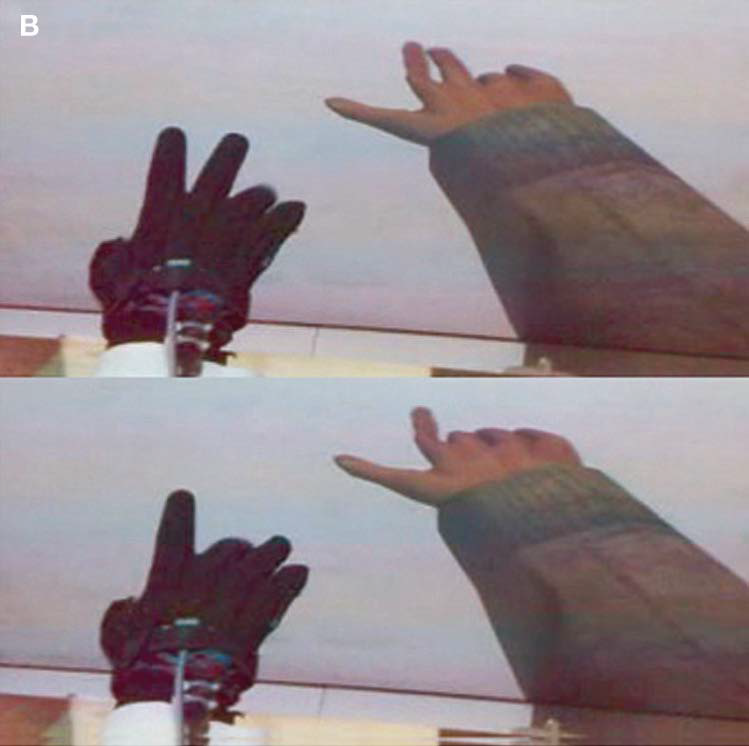
\includegraphics[scale=0.4]{images/biblio/rhiRV}}
   	\caption{\label{fig3} Illusion de la main en caoutchouc en Réalité Virtuelle \cite{sl08}}
\end{figure}


\paragraph{Modification de la perception du corps}

En utilisant la sortie de corps avec des mannequins, Catherine Preston et H. Henrik Ehrsson ont réussi à modifier la satisfaction du corps chez des personnes non atteintes de trouble du comportement alimentaire \cite{pr14}. Pour cela une sortie de corps était réalisée sur les sujets en utilisant un mannequin "maigre" représentant 85\% de la masse corporel du sujet et un mannequin large représentant 115\% de la masse corporel. En utilisant le questionnaire \emph{Body Image States Scale} (BISS) \cite{ca02} qui permet de connaître la satisfaction qu'une personne éprouve par rapport à son corps à l'instant présent, ils ont pu constater une modification dans la satisfaction du corps chez les sujets. Avec la sortie de corps, il a donc été possible chez ces personnes de modifier la satisfaction de leur corps et donc de modifier la perception qu'ils avaient de leur corps. Cependant, l'utilisation de mannequins n'est pas pratique car on ne peut pas changer leurs apparences aisément au niveau de la silhouette. 

\subsubsection{Bilan}
Comme on a pu le voir précédemment, on peut modifier la perception du corps avec la sortie de corps et c'est justement ce que nous souhaitons faire pour aider les personnes atteintes d'anorexie mentale. Seulement l'utilisation de mannequin est limitant, alors qu'avec un modèle 3D d'un corps humain il serait notamment possible de modifier sa silhouette en temps réel. Pour réaliser cela, il faudra également pouvoir capturer les mouvements de la personne et les reproduire avec le modèle 3D. En regardant ce qui a été fait sur la sortie de corps en réalité virtuelle, des sollicitations tactiles sont nécessaires pour créer le phénomène, ce qui signifie qu'il faudra également capturer les mouvements de l'objet (un bâton par exemple) pour réaliser ces actions et reproduire l'objet et ses mouvements dans l'environnement 3D. Cependant, dans le cas de la main en caoutchouc en réalité virtuelle, le fait que la main virtuelle reproduise les mouvements de la vrai main de l'utilisateur permet de se passer des sollicitations tactiles ce qui pourrait aussi être le cas de la sortie de corps. Enfin le dernier point important est la synchronisation, il ne faut pas qu'il y ait de décalage entre ce qui est vu et, soit la sensation de toucher, soit le mouvement effectué, pour créer le phénomène de sortie de corps.

\subsection{Avatar et environnement 3D}
Dans cette section, nous allons voir l'effet que peut avoir un avatar en fonction de son réalisme ainsi que l'impact que peut avoir un environnement virtuel sur notre perception. 
\subsubsection{Apparence de l'avatar}
En utilisant un avatar virtuel, on peut voir apparaitre un effet appelé la \emph{Uncanny Valley} \cite{mo12}. Cet effet représente initialement le fait que dans le domaine de la robotique, plus un robot ressemble à un humain, plus ces défauts gêneront l'utilisateur qui interagit avec lui. Cet effet existe aussi avec les avatar virtuel \cite{mc12} et est accentué lorsque l'avatar réalise des mouvements. Dans cette étude, on peut constater qu'un avatar très réaliste semble familier à l'utilisateur mais qu'il s'agit de l'avatar moyennement réaliste qui semble le moins familier. L'étude regarde aussi l'effet que peut avoir l'apparition d'artefact dans l'animation de l'avatar. Les problèmes d'animations ont moins d'impact lorsque l'avatar n'est pas réaliste et il s'agit de l'avatar moyennement réaliste qui est le plus déplaisant en cas de mauvaise animations. L'interaction avec un avatar ayant une apparence humaine mais pas suffisamment réaliste peut repousser l'utilisateur.
\subsubsection{Perception dans un environnement virtuel}
Pour voir l'impact de la qualité graphique d'un environnement 3D sur la présence ressenti par l'utilisateur, Slater et al. \cite{sla09} on mit des sujets devant un gouffre virtuel, et on analysé la sensation de présence dans l'environnement 3D via questionnaire et les valeurs de conductances de la peau. Suivant les sujets, l'environnement avait des ombres et des réflections dynamiques ou aucunes des deux. Les résultats montre que la présence des ombres et des réflections augmentent ce sentiment de présence.
\subsubsection{Bilan}
Le réalisme de l'apparence de l'avatar peut avoir un impact sur la capacité de l'utilisateur de se lier à lui. Cependant dans le cas d'une sortie de corps où l'utilisateur voit son corps virtuel de dos, rend le visage de l'avatar non visible et ainsi il ne voit pas que l'expression faciale ne corresponde pas à la sienne. Ceci devrait réduire le risque de produire l'effet \emph{Uncanny Valley}. Des critères graphiques comme la présence d'ombre dynamique pour l'avatar pourraient augmenter la présence de l'utilisateur et aider à la création de l'effet de sortie de corps.

\subsection{Modification d'un corps virtuel}
Dans cette partie nous allons voir différentes méthodes pour modifier l'apparence d'un corps virtuel.

\subsubsection{Shape Interpolation}

La \emph{shape interpolation} permet de passer d'un modèle de corps humain à un autre en transformant les deux modèles en des ensembles de points et en calculant entre chaque point correspondant des deux modèles des points intermédiaires \cite{zh09}. Pour pouvoir réaliser cette transformation, il faut d'abord ré-échantillonner les deux modèles pour les transformer en "nuages" de points. Pour cela, un découpage du modèle est effectué en suivant l'axe du squelette du modèle. Par exemple, pour l'avant-bras une série de coupe parallèle va être réalisée en suivant la partie du squelette connectant le coude et le poignet. Le nombre de coupe réalisé sur un membre doit être identique sur les deux modèles. Une fois ceci réalisé, chaque partie du modèle est représentée par un ensemble de tranche. Ensuite le ré-échantillonnage se fait en trois étapes :
\begin{itemize}
\item \'{E}tape 1 : Pour chaque tranche, on calcule un cercle englobant cette partie du corps.
\item \'{E}tape 2 : On divise le cercle en \emph{n} sections, et on crée \emph{n} rayons qui partent du cercle et vont jusqu'au centre de la tranche.
\item \'{E}tape 3 : On crée un point à l'endroit où chaque rayon traverse la surface du modèle.
\end{itemize}

Une fois que les deux modèles ont été transformés en ensemble de points, Il faut alors calculer un ensemble de points intermédiaires via une interpolation linéaire. \`{A} partir de ces points, la surface du modèle intermédiaire peut être créée en effectuant une triangulation. Sur la figure \ref{fig4} on peut voir des modèles créés avec cette technique.
\begin{figure}[!h]
   	\centerline{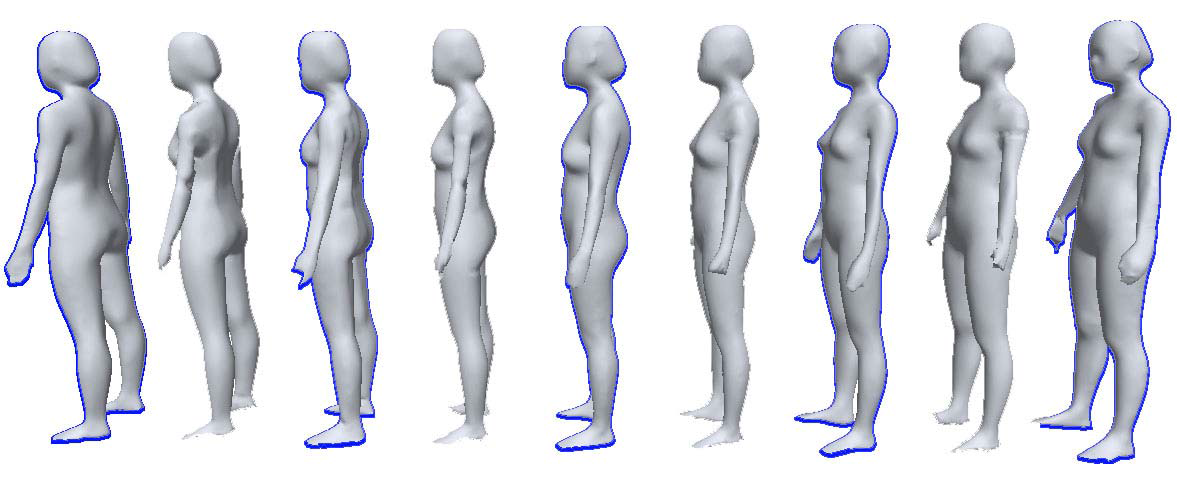
\includegraphics[scale=0.4]{images/biblio/shapeInterpolation2}}
   	\caption{\label{fig4} Modèles de bases (entourés en bleu) et modèles créés par interpolation \cite{zh09}}
\end{figure}
\subsubsection{\emph{Morphing 3D}}
Pour réaliser un \emph{morphing} d'un humain virtuel à un autre en 3D, il faut réaliser plusieurs étapes \cite{le01} :
\begin{itemize}
\item \emph{Morphing} du squelette.
\item \emph{Morphing} de la forme.
\item \emph{Morphing} des coordonnées de la texture.
\item \emph{Morphing} de l'image de la texture.
\end{itemize}
Pour réaliser le \emph{morphing} du squelette et de la forme, il faut que les deux modèles utilisent la même structure pour définir le squelette et la forme. Ensuite les coordonnées du squelette et de la forme peuvent être calculées en utilisant une interpolation linéaire en 3D.
Pour réaliser le \emph{morphing} de la texture, il faut d'abord interpoler les coordonnées de la texture en utilisant une interpolation linéaire en 2D. Le morphing de l'image est réalisé en utilisant des techniques de triangulation. Sur la figure \ref{fig8} on peut voir des modèles créés avec cette technique.
\begin{figure}[!h]
   	\centerline{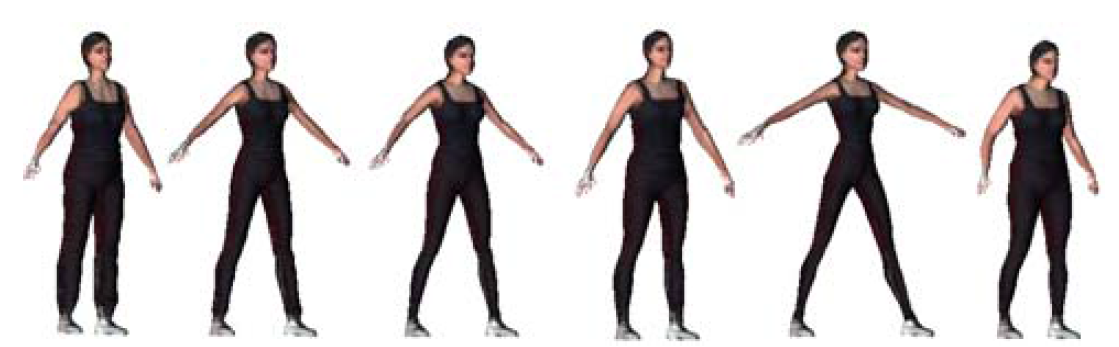
\includegraphics[scale=0.4]{images/biblio/morphing}}
   	\caption{\label{fig8} Modèles avec différentes formes et la même texture \cite{le01}}
\end{figure}
\subsubsection{Modélisation paramétrique}
\subsubsection{Bilan}
La \emph{shape interpolation} permet de passer d'un modèle de corps humain à un autre même si ils ne sont pas définis suivant la même structure. En effet, les points utilisés pour réaliser l'interpolation sont créés avec cette technique. Par contre, il n'y a pas de modification de la texture contrairement au \emph{morphing 3D} et le nombre de calcul est plus important que l'autre technique à cause du calcul des points. Comme les modèles utilisés seront connus, la structure pour définir le squelette et la forme sera identique pour les deux modèles et donc le \emph{morphing 3D} est plus approprié dans notre contexte.

\section{Capture de mouvement}
Dans cette partie, nous allons voir trois grandes classes de système de capture : système mécanique, système magnétique et système optique\cite{kn07}\cite{zo12}. Nous allons d'abord décrire les deux premiers systèmes. Ensuite, nous nous attarderons sur les systèmes optiques en regardant les systèmes optiques avec marqueurs et la \emph{Kinect} puis nous comparerons les performances des deux systèmes. L'étude se limite à ces deux dispositifs car sont ceux disponibles pendant mon stage.
\subsection{Système mécanique}
 Le système mécanique utilise un exosquelette (Voir Figure \ref{fig7}) qui doit être porté par la personne dont on capture le mouvement. Le mouvement est mesuré grâce à des potentiomètres qui sont placés au niveau des articulations ce qui simplifie le traitement de l'information. Son champ d'action est très grand car il n'est relié à aucun appareil externe et il n'y a pas de perturbation au niveau de la mesure. Par contre ce système est très intrusif car l'exosquelette encombre énormément la personne et l'empêche de faire des mouvements rapides.
 \begin{figure}[!h]
    	\centerline{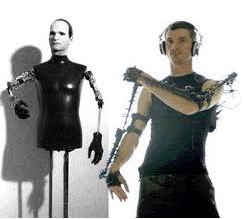
\includegraphics[scale=0.8]{./captureMecaTest}}
    	\caption{\label{fig7} Exemple d'exosquelette}
 \end{figure}
 %\newpage
\subsection{Système magnétique}
Pour ce système, des capteurs sensibles à un champ magnétique produit par un émetteur sont posés sur la personne (Voir Figure \ref{fig9}). La positon et l'orientation des capteurs sont mesurables et la vitesse d'acquisition est très rapide. Ce dispositif est assez peu encombrant par contre il est très sensible à des perturbations pouvant être créées par des objets métalliques ce qui crée des contraintes sur l'environnement où est utilisé ce système.
\begin{figure}[!h]
   	\centerline{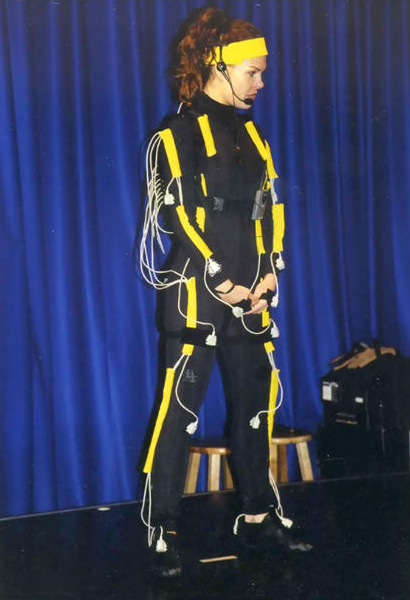
\includegraphics[scale=0.4]{./magne}}
   	\caption{\label{fig9} Combinaison d'un système magnétique}
\end{figure}
\subsection{Système optique}

\subsubsection{Système avec marqueurs}
Dans ce système, l'utilisateur porte une combinaison possédant des marqueurs réfléchissants (Voir Figure \ref{fig5}). Gr\^{a}ce à plusieurs caméras infrarouge, la position de chaque marqueur est récupérée en 3D. Pour cela, chaque caméra émet une lumière infrarouge qui va être réfléchie par le marqueur permettant ainsi d'obtenir une image 2D de celui-ci. En combinant les différentes images obtenues, la position 3D du marqueur peut être calculée. Ce système permet d'avoir une bonne précision et de capturer des mouvements rapides. Ce système est moins encombrant que les deux précédents.
\begin{figure}[!h]
   	\centerline{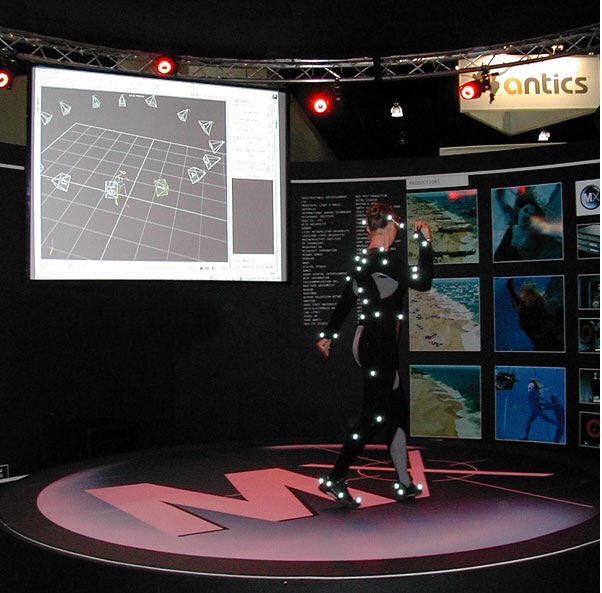
\includegraphics[scale=0.35]{./captureoptic}}
   	\caption{\label{fig5} Dispositif de système optique avec marqueurs}
\end{figure}
\subsubsection{\emph{Kinect}}
La \emph{Microsoft Kinect} est un système de capture de mouvement ne nécessitant pas de marqueurs et embarquant notamment une camera RGB et un capteur de profondeur \cite{ze12}. Le capteur de profondeur permet, en utilisant des rayons infrarouges, d'obtenir l'image de la scène en prenant en compte la profondeur (Voir Figure \ref{fig6}). L'image obtenue est traitée et les formes sont reconnues ce qui permet d'appliquer un squelette sur les formes humaines et ainsi suivre les mouvements.
\begin{figure}[!h]
   	\centerline{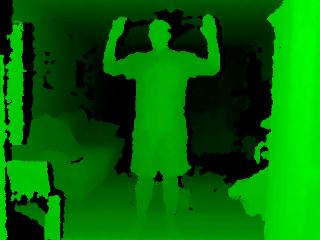
\includegraphics[scale=1.0]{./depthsensor}}
   	\caption{\label{fig6} Exemple d'image obtenu avec le capteur de profondeur}
\end{figure}
\subsubsection{Performances}
Dans l'article \cite{ch12}, les auteurs cherchent à comparer les performances obtenues avec un système optique avec marqueurs \emph{OptiTrack} et la \emph{Kinect} pour leur application d'aide à la réadaptation physique. Dans leur test, le sujet doit effectuer divers mouvements au niveau des mains, des coudes et des épaules qui sont capturés en même temps par le système \emph{OptiTrack} et le système \emph{Kinect}. Ils ont pu constater que la \emph{Kinect} capture très mal les mouvements effectués au niveau des épaules contrairement au système optique avec marqueurs. Cela est dû au fait que la \emph{Kinect} n'utilise qu'une seule caméra contrairement à l'autre système qui en utilise plusieurs (16 dans ce test). En comparant les trajectoires obtenues pour les coudes et mains, ils ont pu voir que les résultats des deux systèmes étaient proches. La latence relative entre les deux systèmes a également été calculée et le système \emph{OptiTrack} était plus rapide de 50 ms. La \emph{Kinect} n'offre pas la possibilité de reconnaitre la position et le mouvement des doigts. La portée de la \emph{Kinect} est d'environ de 0.5 à 4 mètres et la portée optimale est d'environ 1.2 à 3.5 mètres. La distance à laquelle se tient l'utilisateur influence beaucoup la performance du \emph{Kinect} \cite{li12}.

\subsection{Bilan}
Les systèmes optiques avec marqueurs sont rapides et permettent une bonne précision ce qui est nécessaire pour notre projet. Cependant ce système implique le port d'une combinaison avec marqueurs et cela pourrait gêner les utilisateurs dans notre contexte. Comme on a pu le voir, la \emph{Kinect}, bien qu'ayant des performances inférieures à ceux des systèmes optiques avec marqueurs, est suffisamment fiable et rapide. Par contre, la \emph{Kinect} peut ne pas capturer certains mouvements dû à sa seule caméra. Il faudra donc penser au placement de la caméra lors de la capture. Comme la \emph{Microsoft Kinect} est un dispositif plus simple à mettre en place, elle peut être utilisée dans plus d'environnements qu'un système optique avec marqueurs.

\subsection{Synthèse}

Comme nous l'avons vu, les patients atteints d'anorexie mentale doivent prendre conscience de leur maigreur pour que le processus de renutrition puisse aboutir. La sortie de corps, qui consiste à faire croire à une personne qu'un corps virtuel est son vrai corps, pourrait aider efficacement à modifier la perception qu'ils ont de leurs corps. Cette illusion est basée sur le même principe que celle de la main en caoutchouc et comme cette dernière s'est montrée efficace sur les personnes atteintes d'anorexie mentale, on peut en déduire que la sortie de corps est réalisable sur les patients et qu'elle pourrait même être particulièrement efficace.\\

Nous avons vu que réaliser la sortie de corps en réalité virtuelle était possible en créant un conflit entre ce que le sujet voit et ce qu'il ressent physiquement. Ainsi, en créant des stimulations tactiles sur le sujet en le touchant avec un bâton par exemple, pendant qu'il voit les mêmes stimulations tactiles réalisées sur le faux corps, que ce soit son propre corps filmé de dos ou celui d'un mannequin, on peut faire ressentir l'illusion de sortie de corps. Pour la main en caoutchouc, l'illusion est réalisable en réalité virtuelle sans utiliser de stimulation tactile. \`{A} la place, il reproduisait avec la main virtuelle les mouvements que l'utilisateur faisait avec sa vrai main et ils sont réussi à obtenir des résultats similaires. Reproduire les mouvements de l'utilisateur sur le corps virtuel en temps réel pourrait peut-être permettre de créer l'illusion de sortie de corps. \\

L'effet d'appartenance au corps virtuel créé par la sortie de corps est démontré par le fait qu'après l'expérience, le sujet se place plus près de là où il voyait le corps virtuel qu'il ne l'était réellement. De plus, il a été observé que simuler une attaquer sur le faux corps augmente la conductivité de la peau ce qui montre qu'une réponse émotionnelle a lieu lors que le corps virtuel est en "danger". Preston et Ehrsson \cite{pr14} ont également montré que l'utilisation de cette illusion pouvait changer la perception qu'une personne a de son corps et d'en modifier la satisfaction bien que l'utilisation de mannequin leur imposait des limites. Il existe des techniques pour modifier la silhouette d'un corps virtuel comme le \emph{morphing 3D} et réaliser cette modification pendant que le sujet ressent l'illusion de sortie de corps pourrait avoir un impact plus important sur sa perception.\\

Pour capturer le mouvement, \emph{Kinect} est un système simple à mettre en place, il n'y a qu'une seule caméra et il n'y a pas de contrainte sur l'environnement à part la distance à laquelle on se trouve du dispositif. Par contre, la présence d'une seule caméra fait que certains mouvements ne sont pas vus et le dispositif ne capte pas avec autant de précision les mouvements qu'un système optique avec marqueurs. Ce dernier quant à lui, permet d'obtenir des mouvements précis si la personne est équipée de suffisamment de marqueurs et la fréquence d'acquisition des données est élevé. Comme il nécessite plusieurs caméras, il y a moins de risque que certains mouvements ne soit pas vus. En revanche, il s'agit d'un système qui demande plus de matériel et qui est intrusif car la personne doit porter des marqueurs et généralement une combinaison.

\section{Proposition}
Pour créer la sortie de corps dans le but d'aider les patients atteints d'anorexie mentale, nous devons respecter deux critères. Tout d'abord la synchronisation entre ce qui est vu dans le virtuel et perçu dans la réalité est essentiel pour créer le phénomène de sortie de corps en réalité virtuelle. Ensuite, le contexte applicatif du sujet, nous contraint d'utiliser du matériels à bas prix.\\

Pour mettre au point une application permettant d'induire la sensation de sortie de corps, nous allons nous inspirer du principe notamment utilisé par Lopez et al. \cite{bl10} en utilisant un stimuli tactile qui affecte à la fois le vrai corps et le corps virtuel telle que le bâton qui touche le sujet pendant que celui-ci vois une vidéo en direct de lui touché par ce même bâton. Pour avoir un impact sur la perception de l'apparence de son corps, nous allons reprendre l'idée décrite par Preston et al. \cite{pr14}. Dans leur article, ils décrivent la manière dont ils ont pu modifier la satisfaction que les personnes ont de leurs corps grâce à une sortie de corps partielle au niveau du ventre et avec des mannequins de différentes corpulences. Dans notre cas nous souhaitons réaliser cela avec une sortie de corps complète permettant ainsi d'avoir un impact sur la perception qu'ils ont de leurs bras et jambes. Pour obtenir plus de liberté dans l'apparence du corps virtuel et aussi dans sa modification, nous allons réalisé cette sortie de corps dans un environnement virtuel 3D qui sera vu via un casque de réalité virtuelle et des modèles 3D de corps humain.\\

Pour créer la sensation de sortie de corps, nous avons décidés de nous baser sur deux principes, la corrélation visuotactile et la corrélation visuomotrice entre le monde réel et le monde virtuel dans le but de perturber le processus d'intégration multisensorielle.\\

\begin{figure}[!h]
   	\centerline{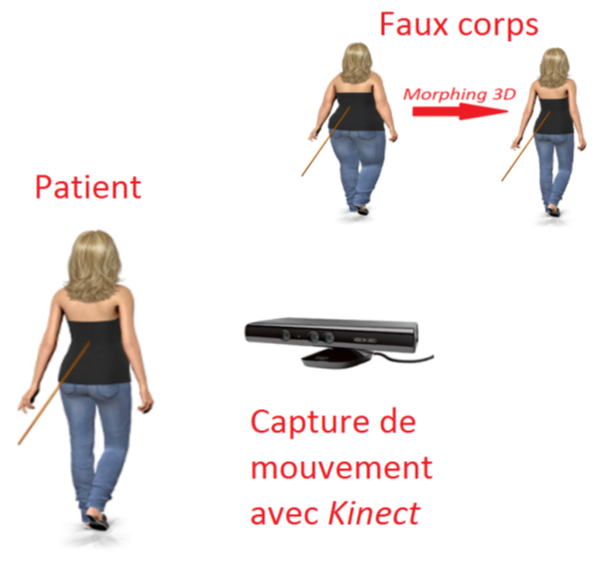
\includegraphics[scale=0.8]{images/schemaProposition}}
   	\caption{\label{fig10} Schéma de l'application proposée}
\end{figure}

La corrélation visuomotrice, c'est à dire le lien entre ce qui est vu et les mouvements que l'on fait, est réalisée grâce à la capture de mouvement en temps réel qui permet à l'avatar de reproduire les mouvements réalisés par l'utilisateur. la corrélation visuotactile, lien entre ce qui est vu et ce qui est ressenti par l'utilisateur, est fait en se servant d'un bâton qui viendra touché le sujet et dans le monde virtuel, un bâton viendra également toucher l'avatar en reproduisant les mouvements du bâton réel. Comme dans certains des travaux vu précédemment, nous avons décidé de choisir le dos pour être la zone sur laquelle seront réalisée les stimulations tactiles. Il faut donc que dans le monde virtuel, l'utilisateur voit son avatar de dos (Voir Figure \ref{fig10}). Ces deux points sont donc réalisés grâce à la capture de mouvement, ceux du sujet et ceux du bâton. La capture de mouvement de l'utilisateur sera réalisée via la \emph{Microsoft Kinect} car elle propose une capture de mouvement de bonne qualité par rapport à son coût. Pour capturer les mouvements du  bâton, nous utiliserons la \emph{Razer Hydra} car elle offre une bonne précision tout en restant abordable et comme l'expérimentateur sera celui qui utilisera cet appareil, le fait qu'il s'agit d'un système intrusif n'est pas un problème.\\

\begin{figure}[!h]
   	\centerline{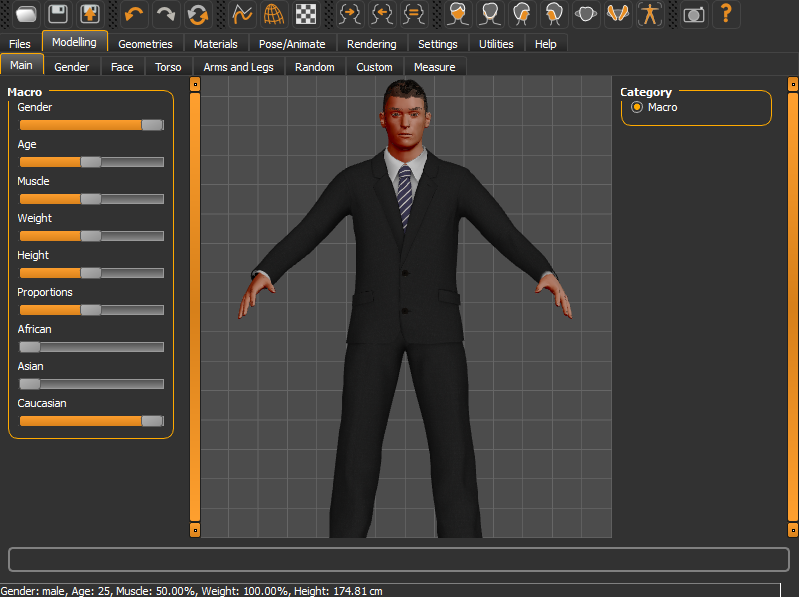
\includegraphics[scale=0.4]{images/makeHuman}}
   	\caption{\label{fig11} Interface de \emph{MakeHuman}}
\end{figure}

Pour l'avatar contrôlé par l'utilisateur, nous avons décidé de proposer aux patients une large gamme de modèles avec les mêmes caractéristiques (cheveux, vêtements, visage ...) mais avec des corpulences différentes. Les différents modèles seront créés avec \emph{MakeHuman}\footnote{www.makehuman.org}. Nous avons choisi ce programme car, en plus d'être open-source et sous licence CC0, il offre un large ensemble d'options pour modifier l'apparence d'un modèle en ce qui concerne la corpulence de son corps (Voir Figure \ref{fig11}). Ainsi il est possible de modifié la masse corporelle et la masse musculaire, ou de modifier chaque membre un par un. Comme tout nos modèles seront proches et fait à partir du même logiciel, il est facile de s'assurer que tout nos avatar aient les mêmes caractéristiques technique tel que le même nombre de points pour définir la forme des modèles et les mêmes textures. On peut aisément utiliser le \emph{Morphing 3D} pour créer la déformation d'un avatar vers un autre.\\

Ainsi la première étape sera que le sujet choisisse l'avatar qui lui ressemble le plus en terme de corpulence puis l'expérimentateur pourra choisir un autre avatar. Ensuite l'utilisateur verra l'avatar choisit de dos dans une simple scène 3D représentant une pièce classique. L'expérimentateur commencera alors à toucher le sujet dans le dos pendant que le bâton virtuel fera la même chose sur l'avatar. En même temps, le corps virtuel se transformera progressivement jusqu'à avoir l'apparence du modèle choisi par l'expérimentateur. 

\section{R\'{e}alisation}
Pour implémenter notre application, nous allons utiliser le moteur Unity\footnote{www.unity3d.com}, un système multiplateforme de création de jeu vidéo développé par Unity Technologies. Ce système comprend un moteur de jeu et un environnement de développement intégré (IDE). L'application sera vu par l'utilisateur à partir d'un casque de réalité virtuelle pour améliorer le sentiment de présence dans le monde virtuel. Pour le casque, nous allons utiliser l'Oculus Rift \cite{oc12} car il s'agit du seul dispositif de ce type disponible sur le lieu de stage.
\subsection{Acquisition des mouvements}
La \emph{Microsoft Kinect} est disponible en deux versions, la première sortie en Novembre 2010 communément appelée \emph{Kinect V1} dont la déclinaison, \emph{Kinect for Windows} qui permet de s'en servir avec un ordinateur, est sortie en Février 2012. La seconde version, \emph{Kinect V2}, est sortie en été 2014. Il existe des différences importantes entre les deux versions, notamment dans le fonctionnement du capteur profondeur \cite{lu15}. En effet, dans la premier version, un motif prédéfini est projeté par rayon infrarouge et la profondeur est calculé en observant les déformations de ce motif. Cependant, comme il existe un espace entre les différents points qui créent le motif, il faut faire une interpolation pour obtenir les valeurs manquantes et le résultat obtenu par le capteur de profondeur peut manquer de précision. Pour la seconde version, \emph{Microsoft} a utilisé une technologie différente basée sur le temps de vol. Des rayons infrarouges sont envoyés dans la zone vue par la \emph{Kinect v2} et la réflexion des rayons est détectée par le capteur de profondeur. \`{A} partir du temps écoulé entre ces deux événements, la profondeur peut être calculée pour chaque pixels qui composent l'image obtenu. Les utilisateurs face à la \emph{Kinect} sont détectés et suivis à partir de l'image obtenu par le capteur de profondeur qui est ensuite traitée pour reconnaitre les formes humaines, ce qui fait que la \emph{Kinect V2} permet une meilleure capture des mouvements que la version précédente. De plus, la version récente capture plus de points sur la personne suivie que la première version, 25 pour la \emph{Kinect V2}(Voir Figure \ref{track}) et 20 pour la \emph{Kinect V1}, nous allons donc, pour capturer les mouvements de l'utilisateur, utiliser la seconde version de la \emph{Microsoft Kinect}.\\

\begin{figure}[!h]
   	\centerline{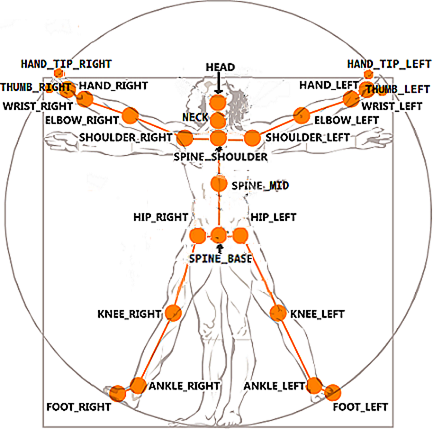
\includegraphics[scale=0.7]{images/kinectTracking}}
   	\caption{\label{track} 25 points reconnus par la \emph{Kinect V2} }
\end{figure}

La \emph{Microsoft Kinect V2} permet d'obtenir la position et l'orientation de chacun des 25 points reconnus sur l'utilisateur. Pour contrôler l'avatar, il n'est pas possible d'utiliser la position des points obtenus car elle dépends en partie de la morphologie de la personne dont les mouvements sont capturés. Cela modifierait la longueur des différents membres de l'avatar et aurait donc un impact négatif sur son apparence. On utilise donc l'orientation des points pour modifier la rotation au niveau des différentes articulations de l'avatar. Pour s'assurer que les valeurs obtenus par la \emph{Kinect} ne sont pas irréaliste, les valeurs sont filtrées pour respecter les rotations permises par les articulation du corps humain.\\

Pour obtenir les mouvements du bâton virtuel, nous utilisons une des deux manettes de la \emph{Razer Hydra}  (Voir Figure \ref{Razer}) à laquelle nous accrochons directement le bâton réel qui servira à toucher l'utilisateur dans le dos. De cette façon, nous pouvons récupérer la position et l'inclinaison de la manette dans un espace en trois dimensions par rapport à la base de la \emph{Razer Hydra}, ce qui correspond également à ceux du bâton. L'appareil étant fait pour le jeu, chacune des manettes possèdent six boutons et un joystick qui nous servent à déplacer le bâton virtuel afin de s'assurer au début de l'application que la position du bâton virtuel correspond bien à celui du bâton réel avant de commencer à toucher la personne dans le dos (Voir Figure \ref{batonAvatar}). Comme la \emph{Razer Hydra} donne la position et l'inclinaison, on peut déplacer le bâton virtuel pour qu'il reproduise les mouvements du bâton réel en obtenant un résultat fluide et fidèle.
\begin{figure}[!h]
   	\centerline{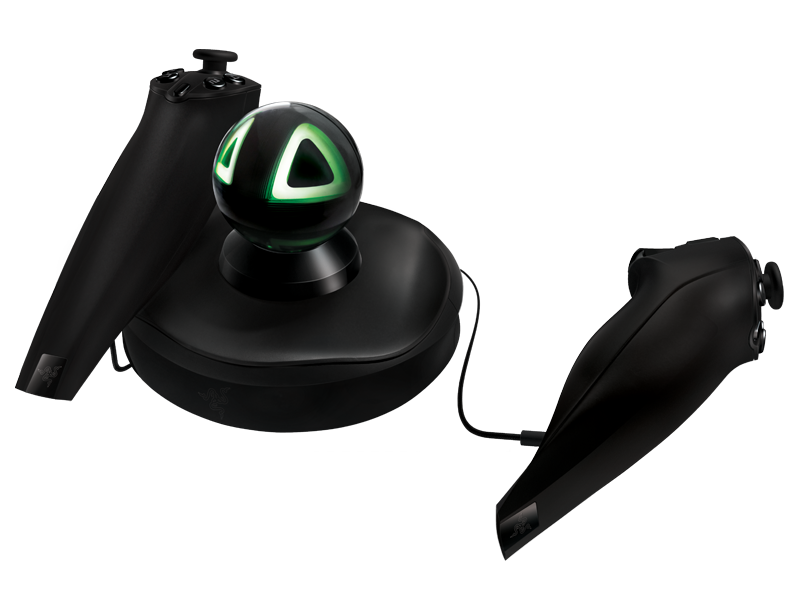
\includegraphics[scale=0.2]{images/biblio/razerHydra}}
  	\caption{\label{Razer} \emph{Razer Hydra}}
\end{figure}
\begin{figure}[!h]
   	\centerline{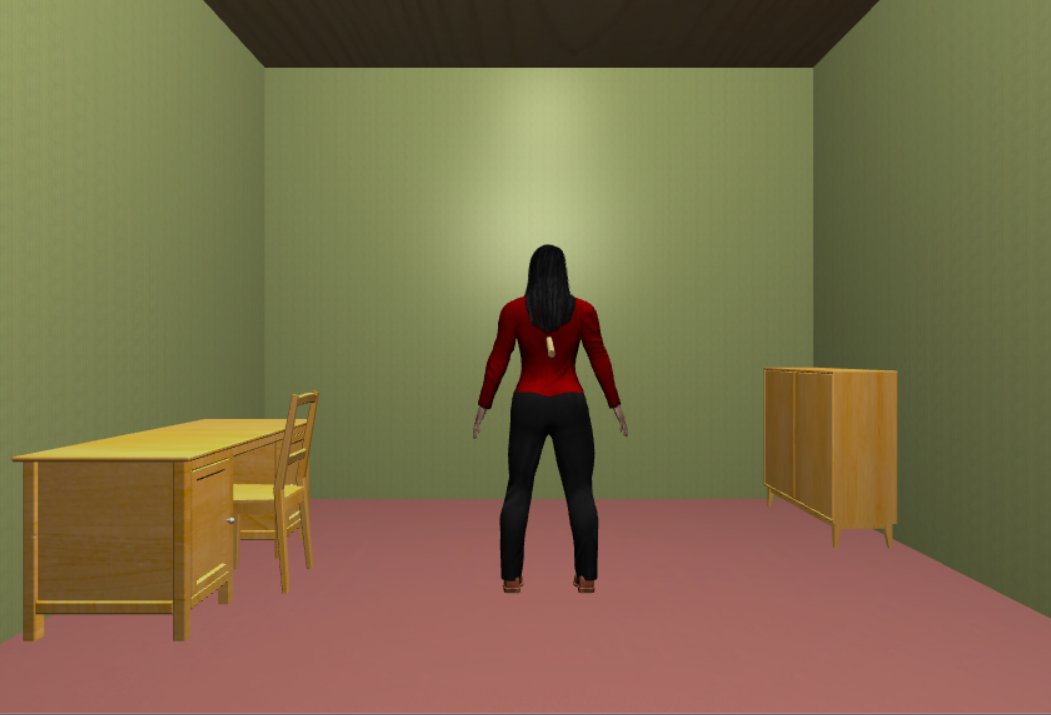
\includegraphics[scale=0.5]{images/avatarBaton2}}
   	\caption{\label{batonAvatar} Avatar touché par le bâton virtuel }
\end{figure}
\subsection{Avatars}
\subsubsection{Création et choix des modèles}
Comme précisé dans la section précédente, nous utilisons \emph{MakeHuman} pour créer nos modèles de personnage. Pour créer de nombreux modèles avec des corpulences différentes, nous avons utilisé deux des paramètres proposé par ce logiciel pour modifier l'apparence : la masse et le muscle. La masse permet donc de modifier le poids de l'avatar et le paramètre muscle permet de changer la musculation de l'avatar. Ces deux paramètres prennent des valeurs entre 0\% et 100\%. On crée ainsi des modèles qui ont 0\%, 25\%, 50\%, 75\% et 100\% de masse et pour chacune de ces valeurs, on prend des valeurs de musculation de 0\%, 25\%, 50\%, 75\% et 100\%. Ce qui nous donne vingt-cinq modèles différents. \emph{MakeHuman} permet de faire des personnages femme et homme et nous créons donc des avatars des deux genres pour convenir à la fois à un utilisateur et une utilisatrice. Lors du lancement de l'application, l'utilisateur est d'abord invité à choisir son avatar parmi les vingt-cinq proposés. Les avatars proposés par l'interface varie en fonction du genre de l'utilisateur (Voir Figure \ref{uiF}). L'utilisateur peut alors sélectionner l'avatar lui ressemblant le plus selon lui en cochant la \emph{checkbox} associée au modèle. L'expérimentateur peut ensuite choisir un autre avatar qui correspond plus à la véritable apparence de l'utilisateur.
\begin{figure}[!h]
   	\centerline{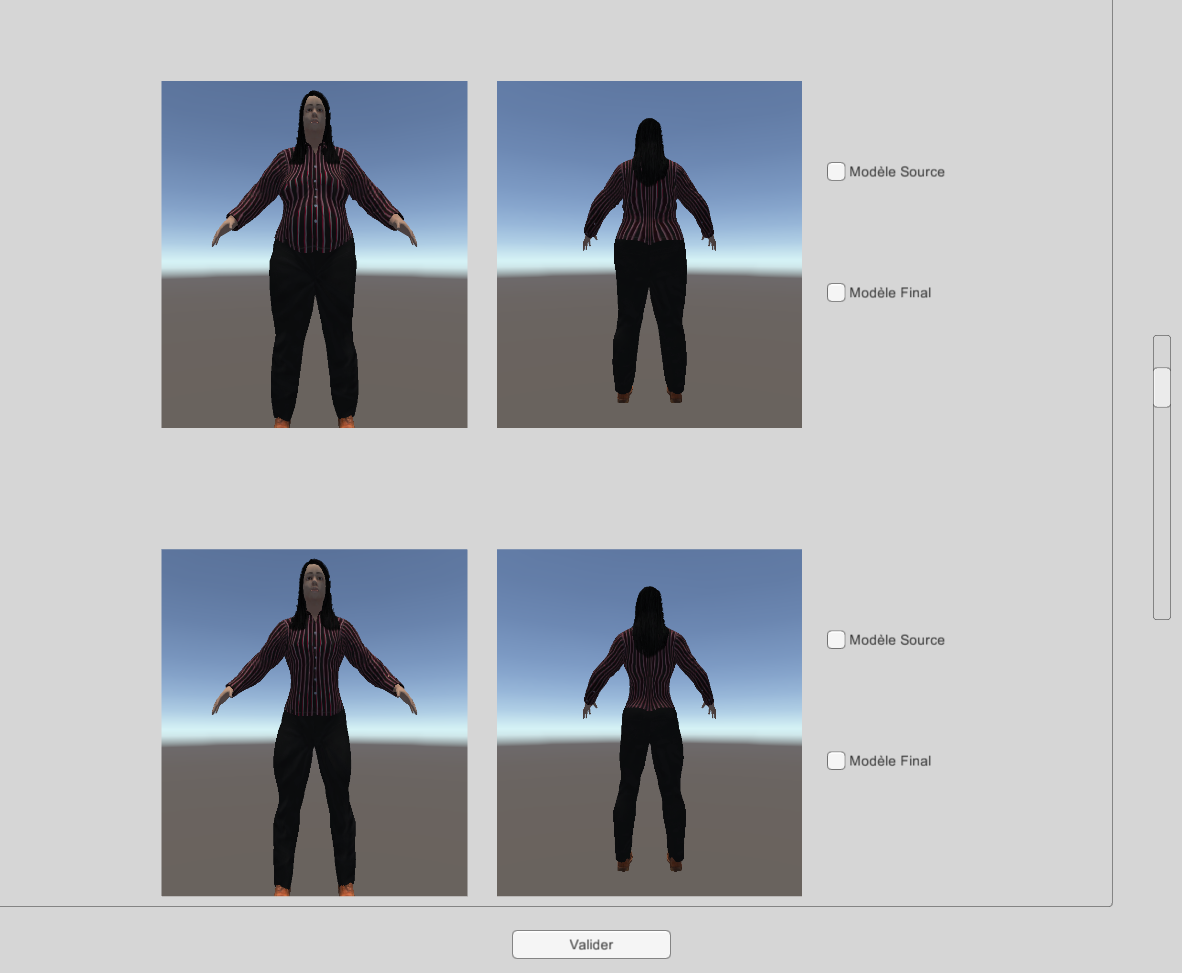
\includegraphics[scale=0.30]{images/interfaceF}}
   	\caption{\label{uiF} Interface pour choisir un avatar féminin }
\end{figure}
\subsubsection{Modification de l'avatar}
Comme nos avatars sont tous créés grâce à \emph{MakeHuman}, nous pouvons nous assurer que chacun de nos modèles est définit de la même manière, le maillage du personnage (\emph{Mesh}) est définit avec le même nombre de point (\emph{Vertex}), ce qui nous permet d'utiliser le \emph{Morphing 3D}, une technique demandant peu de calcul et donc bien adaptée au temps réel. Durant notre modification, seul la forme de l'avatar change, c'est-à-dire que seul le maillage, qui permet de créer la forme du modèle, est modifié. Les textures restent les mêmes durant la modification. Le \emph{Morphing 3D} est réalisé via un calcul d'interpolation linéaire. Pour cela on calcule chaque point intermédiaire de cette façon :
\begin{center}
$P = \alpha*P_i + (1-\alpha)*P_j$, avec $0<\alpha<1$
\end{center}
Avec $P$ qui est le point intermédiaire, $P_i$ et $P_j$ sont les points équivalents appartenant respectivement au modèle de départ et au modèle d'arrivé. Avec le moteur, nous avons défini que le calcul serait réalisé toute les 20ms. Nous souhaitons que la modification se fasse sur la durée d'une minute, ce qui fait que lors de notre \emph{Morphing 3D}, un total de 3000 modèles intermédiaires sont calculés et vus par l'utilisateur. Le but qu'on cherche à atteindre avec ce paramétrage et ce nombre de modèle intermédiaire calculé, est d'obtenir une modification suffisamment subtile pour que l'utilisateur ne se rende pas tout de suite compte que son avatar est en train de changer mais plutôt qu'il se rende compte après la modification ou vers la fin que son avatar a changé. Sur la Figure \ref{morphingGhost}, on peut voir un avatar après avoir été modifié et en transparent apparait la forme d'origine.

\begin{figure}[!h]
   	\centerline{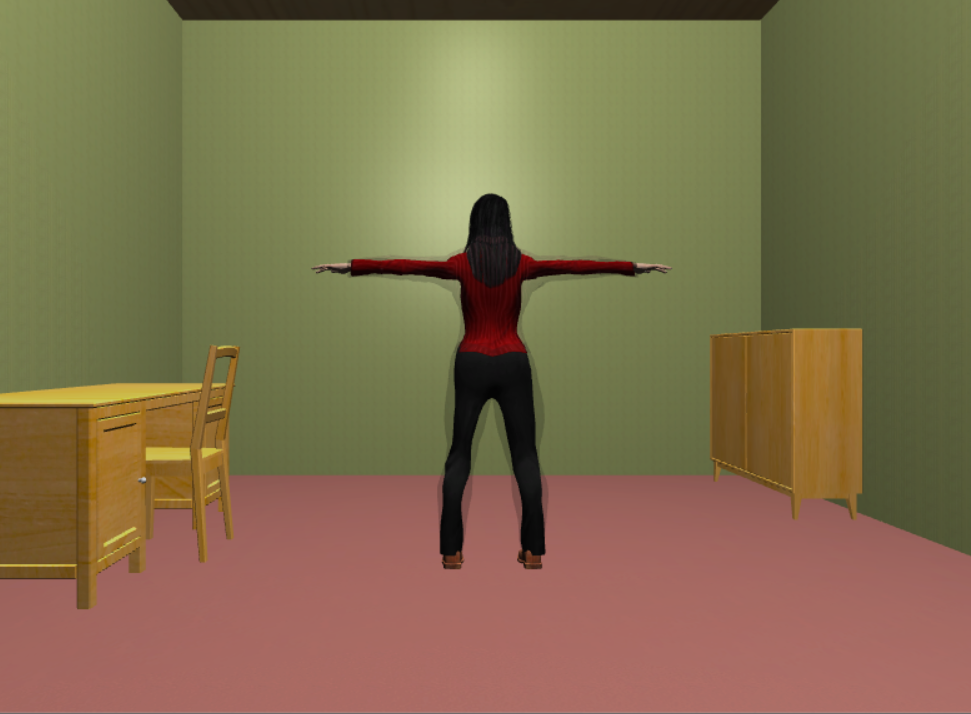
\includegraphics[scale=0.5]{images/morphingGhost2}}
   	\caption{\label{morphingGhost} Modèle après modification avec apparence d'origine en transparence }
\end{figure}

\section{Méthodes d'évaluation}

Pour évaluer l'application, nous allons réaliser une étude dans laquelle on modifie deux facteurs, la présence ou non de la stimulation tactile et la présence ou non de la modification du corps. La raison pour laquelle nous modifions ces deux facteurs est que nous voulons tester l'impact de ces deux paramètres et pour cela, il nous faut des conditions permettant d'obtenir des mesures de contrôle afin d'obtenir une base pour comparer les résultats. Ceci nous donne les quatre conditions suivantes :
\begin{itemize}
\item Condition 1 : Le bâton virtuel se déplace automatiquement, le sujet n'est pas touché par le bâton réel. Le corps n'est pas modifié.
\item Condition 2 : Le bâton virtuel se déplace automatiquement, le sujet n'est pas touché par le bâton réel. Le corps est modifié.
\item Condition 3 : Le sujet est touché par le bâton réel et le bâton virtuel reproduit les mouvements du bâton réel. Le corps n'est pas modifié.
\item Condition 4 : Le sujet est touché par le bâton réel et le bâton virtuel reproduit les mouvements du bâton réel. Le corps est modifié.
\end{itemize}
Pour chaque conditions, la durée d'utilisation de l'application est de 60 secondes. Les différences entre les conditions 1 et 2 et les conditions 3 et 4, permettent d'obtenir des résultats pour voir l'influence de la modification du personnage. Dans les deux premières conditions, le bâton virtuel est présent mais il bouge automatiquement et le sujet n'est pas touché par le vrai bâton en même temps. Dans ces deux conditions, le sujet voit son avatar être touché par un bâton virtuel au niveau du dos avec des mouvements de haut en bas. Alors que dans les deux dernières conditions, le bâton virtuel reprend les mouvements du bâton réel et le sujet est donc touché par le bâton en même temps que son avatar (Voir Figure \ref{batonAvatarS}). Les différences entre les deux premières conditions et les deux dernières conditions, permettent de voir le réel impact du bâton virtuel qui reprend les mouvements du bâton réel et qui permet de créer la sensation de sortie de corps en réalité virtuelle.\\

Chaque sujets utilisent l'application suivant les quatre conditions. Entre chaque conditions, leur capacité à se localiser dans l'espace et leur perception de la largeur de leur corps sont mesurées et un questionnaire leur est donné. Durant l'expérience et les mesures, les participants portent un casque de réalité virtuelle \emph{Oculus Rift DK2} et un casque audio pour ne pas être dérangé par les bruits extérieurs. Tout d'abord, le sujet choisi l'avatar qui lui est le plus proche en terme de corpulence puis l'expérimentateur choisi un autre avatar. Ensuite, un premier essai est réalisé, dans le but de présenter l'expérience, où les participants peuvent tester l'application en bougeant leur avatar et voir le bâton virtuel, ainsi que pour montrer comment sont réalisées les mesures. On profitent de cette session d'entrainement pour obtenir les valeurs de comparaison pour chaque mesures. Afin que nos mesures ne soit pas faussées par le fait que le sujet peut s'habituer à l'exercice, particulièrement pour la localisation dans l'espace, les conditions peuvent être faites dans deux ordres différents : 1,2,3,4 et 3,4,1,2. Ainsi, on peut savoir si ce sont réellement les conditions qui impactent les résultats obtenus.
\begin{figure}[!h]
   	\centerline{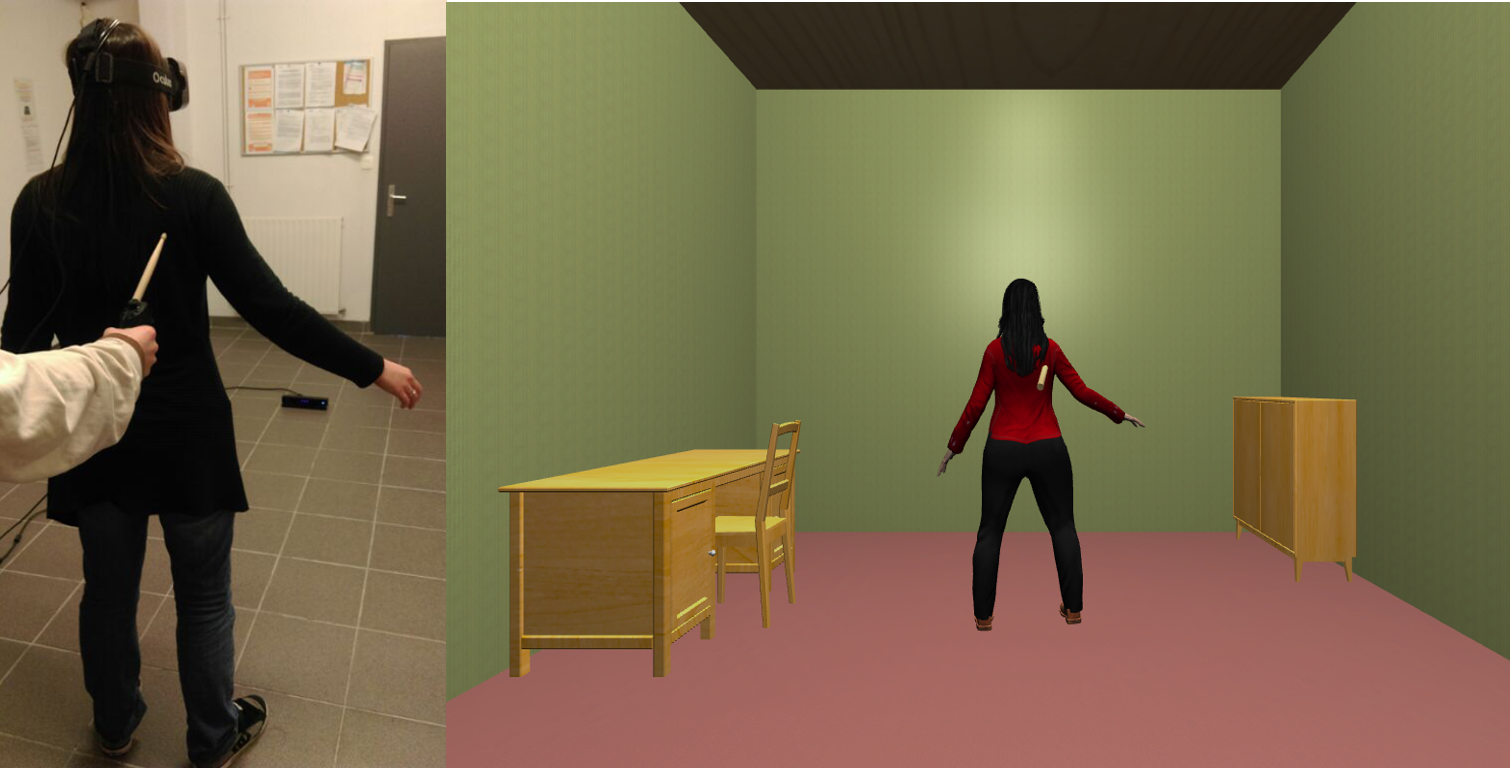
\includegraphics[scale=0.35]{images/doubleView2}}
   	\caption{\label{batonAvatarS} Utilisateur et avatar touchés par le bâton }
\end{figure}
\subsection{Localisation dans l'espace}
Pour mesurer la capacité à se localiser dans l'espace, le sujet doit marcher sur place pendant que l'expérimentateur le recule d'une distance constante entre chaque essai. On demande ensuite au participant de se replacer là où il était. Durant toute cette mesure, le sujet garde le casque et ne vois donc pas devant lui. On mesure ensuite la distance entre l'endroit où le sujet se replace et l'endroit où il était réellement. Pour cette mesure, on s'inspire de celle réalisée par Blank et al. \cite{bl10} dont le but est d'évaluer objectivement si le sujet à ressenti une illusion de sortie de corps.
\subsection{Perception de la largeur du corps}
\begin{figure}[!h]
   	\centerline{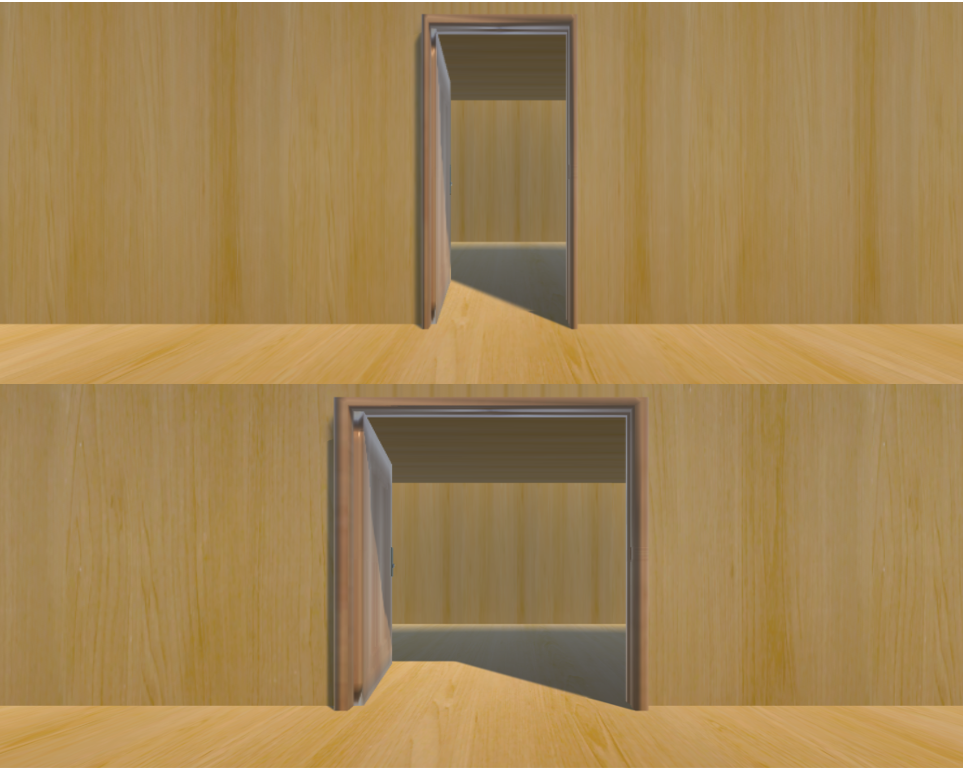
\includegraphics[scale=0.25]{images/doubleDoor3}}
   	\caption{\label{figDoor} Deux portes de largeur différentes }
\end{figure}
Pour connaître la perception implicite que le sujet a de la largeur de son corps, on réalise une mesure proche de celle faite par Guardia et al. \cite{gu10}. Le sujet voit via son casque de réalité virtuelle une série de trente portes qui peuvent avoir six largeurs différentes (Voir Figure \ref{figDoor}). Ainsi le sujet voit à cinq reprise chaque différente porte, et on s'assure que la même porte n'est pas affiché deux fois de suite. Pour chaque porte, le sujet doit dire si il peut passer à travers la porte sans avoir besoin de tourner les épaules. l'ordre des portes est aléatoire et donc différent à chaque mesure.

\subsection{Questionnaire}
Nous avons créés plusieurs questionnaires en fonction des conditions de l'expérimentation. Les participants doivent répondre à chaque question en utilisant une échelle à sept valeurs allant de -3 à 3, avec 3 signifiant 'pas du tout d'accord' et 3 'tout à fait d'accord'. Pour l'élaboration de nos questionnaires, nous nous somme inspirés de ceux fait dans d'autre étude sur la sortie de corps comme Lenggenhager et al. \cite{le07} auxquelles, nous avons rajouter d'autres questions plus spécifiques à notre expérience.Dans le questionnaire pour les conditions 3 et 4 (Voir Annexe \ref{questionnaires2}), trois questions ont pour but de mesurer la sortie de corps selon le ressenti du sujet :
\begin{itemize}
\item Q1 : j'ai eu l'impression de me sentir touché(e) au même endroit qu'était touché le corps virtuel par le bâton.
\item Q2 : j'ai eu l'impression que la sensation d'être touché(e) a été causée par le bâton qui touché le corps virtuel.
\item Q3 : j'ai eu la sensation que le corps virtuel était mon corps.
\end{itemize}

On ajoute d'autres questions, notamment une qui permet d'avoir le retour sur la synchronisation entre réel et virtuel pour le bâton, et deux autres dont on pourra voir si les résultats seront en corrélation avec les résultats de la localisation dans l'espace : 
\begin{itemize}
\item Q4 : j'ai eu l'impression que mon corps (réel) a dérivé vers l'avant (vers le corps virtuel).
\item Q7 : il m'a semblait que visuellement le corps virtuel a dérivé vers l'arrière (vers le corps réel).
\end{itemize}
Ainsi, si dans la mesure de la localisation dans l'espace, le sujet se replace moins loin ou plus loin de là où il se trouvait réellement, on pourra voir si cela se reflète dans ces réponses ou inversement. Pour le questionnaire des conditions 1 et 2 (Voir Annexe \ref{questionnaires1}), on retrouve les même questions que dans le questionnaire décrit précédemment sans celle sur la synchronisation du bâton et la Q2. car dans ces conditions il n'y a pas de bâton réel qui touche le sujet. On garde les questions Q1. et Q3. car cela nous permet d'avoir une base de comparaison pour voir l'effet lorsque le bâton réel et virtuel font les même mouvements.\\

Le questionnaire de fin (Voir Annexe \ref{questionnaires3}) permet d'obtenir des informations en ce qui concerne l'habitude des participants à interagir avec un environnement virtuel. Il permet également de recueillir des retours sur la qualité de l'application en ce qui concerne l'apparence de l'avatar, réalisme et aussi si il y avait une vrai impression de ressemblance pour la corpulence, et également pour tout ce qui concerne la capture du mouvement que ce soit pour l'avatar ou pour le bâton. Ces informations supplémentaire pourront nous aider à voir l'impact des aspects techniques mis en place sur les résultats obtenus.



\newpage 
\section{Conclusion et Perspectives}
Dans ce rapport, nous avons cherché à proposer une nouvelle solution pour aider les personnes atteintes d'anorexie mentale. Pour cela, nous nous sommes intéressés au phénomène de sortie de corps en réalité virtuelle. L'illusion de sortie de corps permet de faire croire à une personne qu'un corps virtuel est son vrai corps, et a réussi, chez des personnes en bonne santé, à modifier la satisfaction qu'ils avaient de leur corps. De plus, les expériences menés sur l'illusion de la main en caoutchouc, reposant sur le même principe que celle de sortie de corps, ont montrés qu'elle fonctionnait très bien sur les patients atteints d'anorexie mentale. Nous avons pu voir que l'illusion se crée en mettant en place une corrélation entre ce qui se passe dans le monde réel et ce qui se passe dans le monde virtuel. Pour cette raison, la synchronisation entre ce qui se passe dans le réel et le virtuel est très important.\\

Pour définir notre proposition afin d'aider les patients atteints d'anorexie mentale, nous nous somme inspirés des travaux sur la sortie de corps comme ceux permettant de créer l'illusion de sortie de corps grâce à une stimulation tactile sur le dos à la fois sur le sujet et sur l'avatar qui le représente dans le monde virtuel et celui permettant de changer la satisfaction du corps avec une sortie de corps partielle au niveau du ventre. Notre but est de changer la perception du corps entier et non pas d'une seule partie d'une corps donc nous voulons utiliser une illusion de sortie de corps complète et pour offrir plus de possibilité sur la modification du corps virtuel, nous proposons de réaliser tout cela dans un environnement complètement virtuel.\\

Comme à terme, l'objectif est de permettre au psychiatre du CHU de Brest d'utiliser ce qui a été réalisé dans le traitement des personnes souffrants d'anorexie mentale, nous avons cherché a respecter la contrainte d'utiliser du matériel à bas coût et accessible au grand public. Nous avons donc choisi deux appareils avec un bon rapport prix/précision pour faire la capture de mouvement : la \emph{Kinect V2} pour capturer les mouvements de l'utilisateur et la \emph{Razer Hydra} pour capturer les mouvements du bâton.\\

Afin de tester l'application réalisée, une méthode d'évaluation a été définie. Cette méthode a pour but de mesurer la présence et l'effet du phénomène de sortie de corps ainsi que l'effet de la modification du corps. Que ce soit lorsque la sortie de corps et la modification du corps ont lieu ensemble ou non.\\

Dans la suite du stage, nous ferons passer les expériences en suivant la méthode mise en place pour voir le résultat obtenu avec cette application. Cette évaluation commencera d'abord en prenant pour sujet des personnes travaillant dans le laboratoire de recherche. Ceci nous permettra de mettre en évidence la présence de modifications à réaliser pour améliorer l'application et nous donnera un premier aperçu de l'effet sur la perception de son propre corps. Si les résultats sont positifs, avec l'aide des psychiatres du CHU de Brest, nous pourrons étendre ces expérience à certain de leurs patients atteints d'anorexie mentale.\\

Actuellement, l'utilisateur choisit son avatar parmi une liste qui lui est proposée. Cette liste a pour but de proposer une large variété d'avatar a la corpulence différente mais leurs visages par exemple reste le même et il est impossible de proposé toute les corpulences possibles. L'une des possibilité serait donc de faire un scan 3D de la personne pour créer son avatar virtuel avec la \emph{Kinect V2} comme l'ont fait Cheng et al. \cite{ch15}. Une autre possibilité serait d'implémenter directement dans l'application une interface permettant de réaliser la même chose que \emph{MakeHuman}. Ainsi la première étape pour le patient sera de réaliser son avatar.

 %La sortie de corps, qui consiste à faire croire à une personne qu'un corps virtuel est son vrai corps, pourrait aider efficacement à modifier la perception qu'ils ont de leurs corps. Cette illusion est basée sur le même principe que celle de la main en caoutchouc et comme cette dernière s'est montrée efficace sur les personnes atteintes d'anorexie mentale, on peut en déduire que la sortie de corps est réalisable sur les patients et qu'elle pourrait même être particulièrement efficace.
\newpage 
\begin{thebibliography}{10}

\bibitem{ri11}
  	Riva, G., (2011). The Key to Unlocking the Virtual Body: Virtual Reality in the Treatment of Obesity and Eating Disorders. Journal of Diabetes Science and Technology. Volume 5, Issue 2.
  			
\bibitem{ri13}
	Ferrer-García, M., Gutiérrez-Maldonado, J., Riva, G. (2013). Virtual reality based treatments in eating disorders and obesity: A review. Journal of Contemporary Psychotherapy, 43, 207-221.
	
\bibitem{gu10}
 	Guardia, D., Lafarguea, G., Thomas, P., Dodin, V., Cottencin, O., \& Luyat, M. (2010). Anticipation of body-scaled action is modified in anorexia nervosa. Neuropsychologia, Volume 48, Issue 13, Pages 3961-3966
 		
 \bibitem{lu14}
 	Luyat, M. (2014). Les apports de la psychologie cognitive et de la neuropsychologie dans la compréhension de l'anorexie mentale. Journal de thérapie comportementale et cognitive, 24, 114-121.
 	
 \bibitem{Bo98}
 	Botvinick, M., \& Cohen, J. (1998). Rubber hands ‘feel’ touch that eyes see. Nature, 391, 756.
 	
  	
 \bibitem{bl10}
 	Lopez, C., \& Blanke, O. (2010). Quand l'esprit met le corps à distance. La Recherche, 439, 48-51.
 	
 \bibitem{eh07}
 	Ehrsson H. H. (2007). The experimental induction of out-of-body experiences. Science , 317-1048.
 
 \bibitem{le07}
 	Lenggenhager, B., Tadi, T. Metzinger, T., \& Blanke, O. (2007). Video ergo sum: manipulating bodily self-consciousness. Science, 317, 1096–1099
 	
 
 \bibitem{sl09}
  	Mel Slater, M., Daniel Perez-Marcos, D., H. Henrik Ehrsson, H. H., \& Maria V. Sanchez-Vives, M. V. (2009).Inducing illusory ownership of a virtual body. Frontiers in Neuroscience, 3(2), 214-220.
  	
 \bibitem{sl08}
  	Slater, M., Spanlang, B., Frisoli, A., \& Sanchez-Vives, M.V. (2008). Virtual hand illusion induced by visual- proprioceptive and motor correlations. PLoS ONE 5(4): e10381.
   	
 \bibitem{pr14}
  	Preston, C., \& Ehrsson, H. H. (2014). Illusory changes in body size modulate body satisfaction in a way that is related to non-clinical eating disorder psychopathology. PLoS ONE 9(1): e85773.
  	
 \bibitem{ca02}
 	Cash, T. F., Fleming, E. C., Alindogan, J., Steadman L., \& Whitehead, A. (2002) Beyond Body Image as a Trait: The Development and Validation of the Body Image States Scale. Eat Disord: J Treat Prevent 10: 103–113.
 
 \bibitem{mo12}	
 	Mori, M.; MacDorman, K.F.; Kageki, N., "The Uncanny Valley [From the Field]," Robotics \& Automation Magazine, IEEE , vol.19, no.2, pp.98,100, June 2012 doi: 10.1109/MRA.2012.2192811
 	
 \bibitem{mc12}	
 	McDonnell, R., Breidt, M., \& Bülthoff, H. H. (2012). Render me real?: investigating the effect of render style on the perception of animated virtual humans. ACM Transactions on Graphics (TOG), 31(4), 91.
 	
 %\bibitem{mi13}
 %	Miles, H.C.; Pop, S.R.; Watt, S.J.; Lawrence, G.P.; John, N.W.; Perrot, V.; Mallet, P.; Mestre, D.R., "Investigation of a Virtual Environment for Rugby Skills Training," Cyberworlds (CW), 2013 International Conference on , vol., no., pp.56,63, 21-23 Oct. 2013
 %	doi: 10.1109/CW.2013.45
 	
 %\bibitem{mi10}
 %	Michael Geuss, Jeanine Stefanucci, Sarah Creem-Regehr, and William B. Thompson. 2010. Can I pass?: using affordances to measure perceived size in virtual environments. In Proceedings of the 7th Symposium on Applied Perception in Graphics and Visualization (APGV '10). ACM, New York, NY, USA, 61-64. DOI=10.1145/1836248.1836259 http://doi.acm.org/10.1145/1836248.1836259 
 	
 \bibitem{sla09}
 	Slater, M., Khanna, P., Mortensen, J., Insu Yu, "Visual Realism Enhances Realistic Response in an Immersive Virtual Environment," Computer Graphics and Applications, IEEE , vol.29, no.3, pp.76,84, May-June 2009 doi: 10.1109/MCG.2009.55
 	
 \bibitem{zh09}
 	Zhong, Y. Q., Liu, H. Y., Jiang, J. F., \& Liu L. (2009). 3D Human Body Morphing Based on Shape Interpolation. The 1st International Conference on Information Science and Engineering, p1027-1030.
 	
 \bibitem{le01}
	 Lee, W., Magnenat-Thalmann N. (2001). Virtual Body Morphing Computer Animation, The Fourteenth Conference on Computer Animation. Proceedings, p158-166
 	
 \bibitem{kn07}	
 	Knossow, D. (2007).Paramétrage et Capture Multicaméras du Mouvement Humain. Human-Computer Interaction. Institut National Polytechnique de Grenoble - INPG.
 	
 \bibitem{zo12}
 	Zong, C. (2012). Systèeme embarquée de capture et analyse du mouvement humain durant la 	marche. Automatic. Université Pierre et Marie Curie - Paris VI.
  	
  \bibitem{ku12}
  	Kuntz, S., \& Cíger, J. (2012). Low-cost and home-made immersive systems. The International Journal of Virtual Reality, 11(3), 9-17.
  	
  \bibitem{ze12}	
  	Zhang, Z. (2012). Microsoft Kinect Sensor and Its Effect. MultiMedia, IEEE, vol. 19, no.2, pp. 4-10
 	
 \bibitem{ch12}	
 	Chang, C., Lange, B., Zhang, M., Koenig, S., Requejo, P., Somboon, N., Sawchuk, A. A., \& Rizzo A. A. (2012). Towards Pervasive Physical Rehabilitation Using Microsoft Kinect. In International Conference on Pervasive Computing Technologies for Healthcare (Pervasive-Health), p159-162.
 	
  \bibitem{li12}
 	 Livingston, M. A., Sebastian, J., Ai, Z., \& Decker, J. W. (2012). Performance Measurementsfor the Microsoft Kinect Skeleton. Proc. IEEE Virtual Reality Workshops, pp.119 -120.13
  
  \bibitem{oc12}
  	Oculus, V. R. (2012). Oculus Rift. Available from WWW: http://www. oculusvr. com/rift.
  
  \bibitem{lu15}
  	Lun, R., \& Zhao, W. (2015). A Survey of Applications and Human Motion Recognition with Microsoft Kinect. International Journal of Pattern Recognition and Artificial Intelligence.
  	
  \bibitem{ch15}
  	Chen G., Li J., Wang B., Zeng J., Lu G., and Zhang D. (2015) Reconstructing 3D human models with a Kinect, Comp. Anim. Virtual Worlds, doi: 10.1002/cav.1632.
  	
\end{thebibliography}


%\bibliographystyle{plain}
%\bibliography{Reference}
\appendix
\section{Questionnaires \label{questionnaires}}
\subsection{Questionnaire 1er et 2ème conditions \label{questionnaires1}}
\begin{figure}[!h]
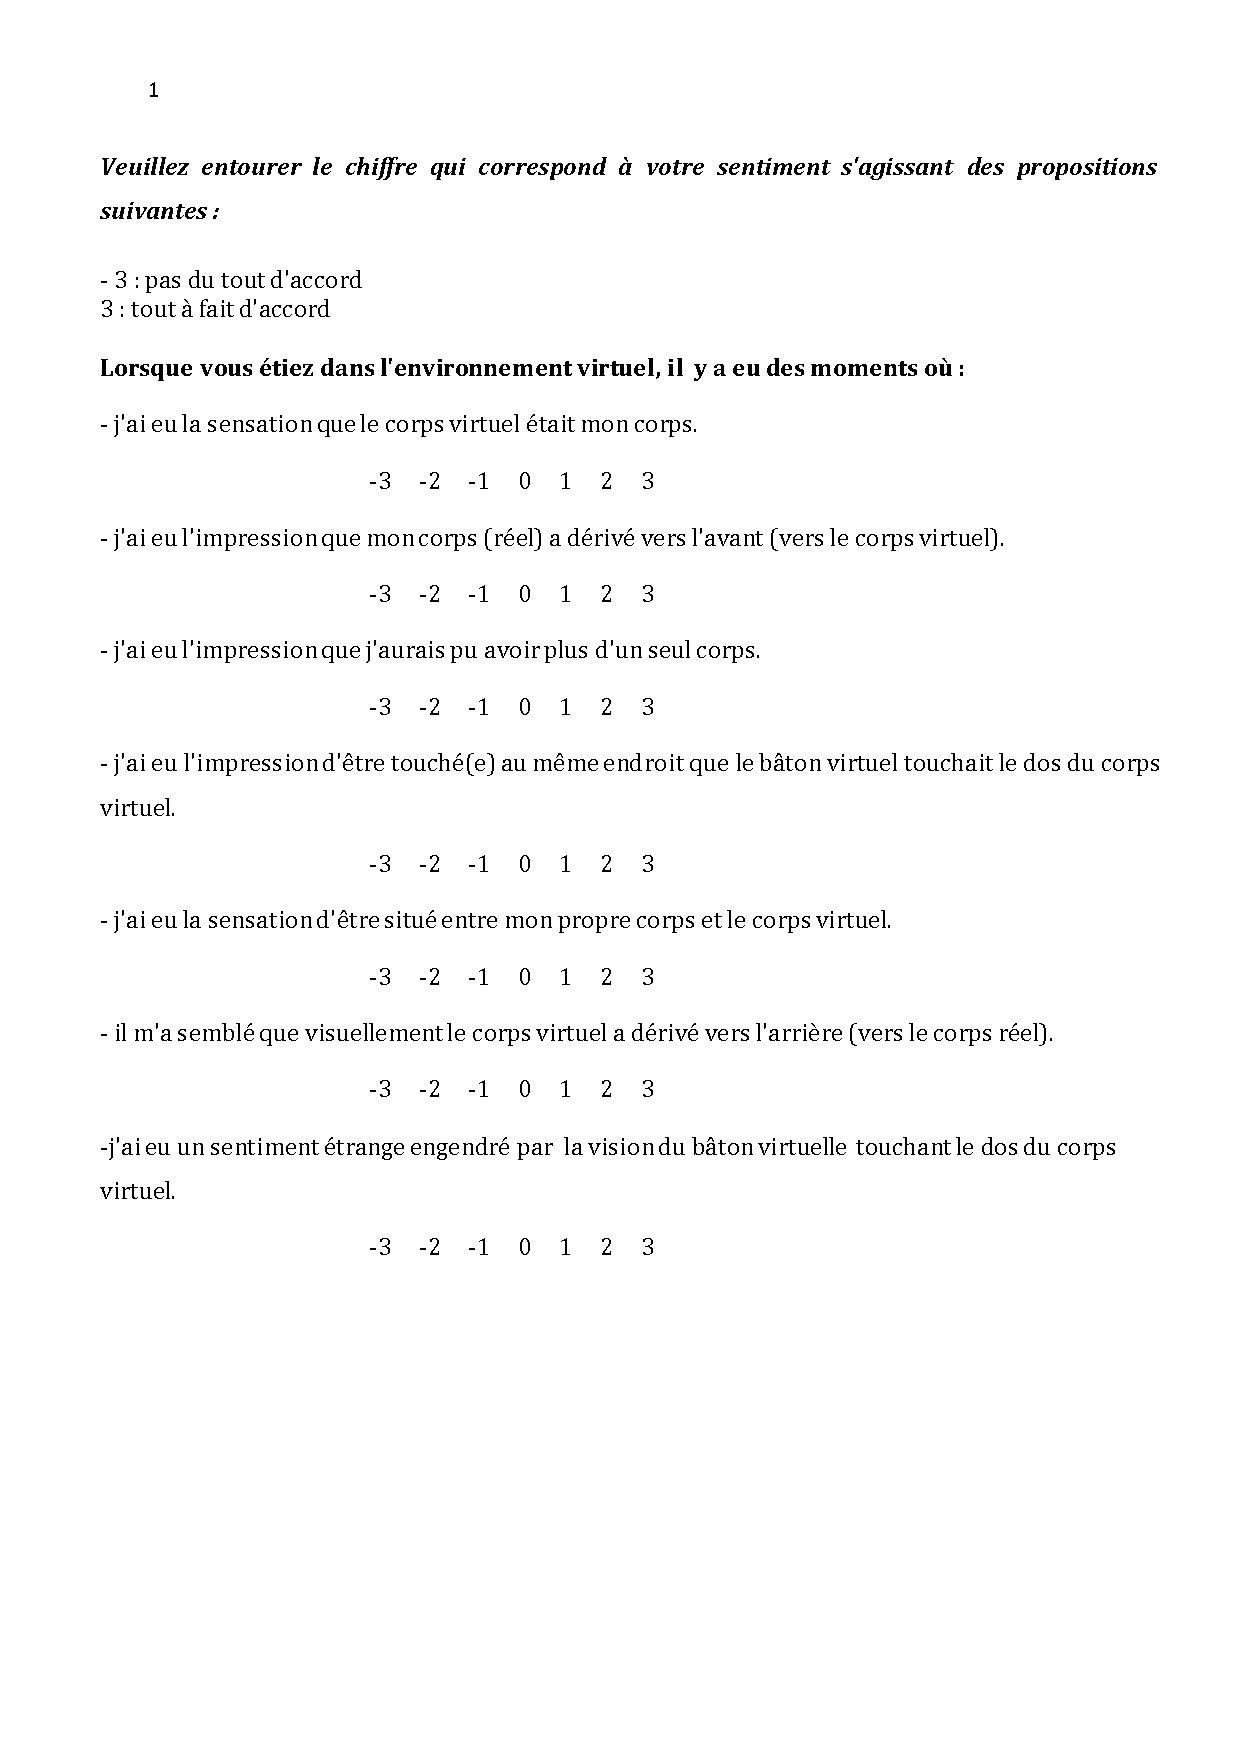
\includepdf[pages={1},offset=0cm -1.5cm]{Questionnaire.pdf}
\end{figure}
\newpage
\subsection{Questionnaires 3ème et 4ème conditions \label{questionnaires2}}
\begin{figure}[!h]
\includepdf[pages={3}]{Questionnaire.pdf}
\end{figure}
\newpage
\subsection{Questionnaire final \label{questionnaires3}}
\begin{figure}[!h]
\includepdf[pages={5}]{Questionnaire.pdf}
\end{figure}
\newpage
\begin{figure}[!h]
\includepdf[pages={6}]{Questionnaire.pdf}
\end{figure}
%\chapter{Doc}
\end{document}
